\subsection{Linkages}
%graph -> G = (V,E)
%linkage -> (G,l)
%embedding -> 
There are two parts to a linkage, the graph and the edge length mapping.   A \textit{graph} is an 
ordered pair $G = (V,E)$ comprising of a set $V$ of vertices or together with a set $E$ of edges or 
lines.  For every edge $e \in E$, there is a distinct pair of vertices in $V$ that it represents, 
$(u,v) \in E$.  While graphs can have vertices that may not correspond to any edges, we rule out 
this possibility for linkages.  The edge length assignement mapping of a linkage is $l: E \mapsto 
\bbr^+$. A linkage is still an abstract combinatorial structure until an \textit{embedding} on the 
graph of the linkage is posed, i.e. $\Pi : V \mapsto \bbR^{2}$. $\Pi$ has the \textit{proper 
embedding} property, if for every edge $(u,v) \in E$ such that $l\left( \left(u,v\right) \right) 
= \left\vert \Pi(u) - \Pi(v) \right\vert$ is true. The \textit{realization} of the the linkage is 
said to be the range $\Pi$, i.e. $\Pi(V)$.  Without loss of generality, for this paper, we focus on 
linkages that have simple planar graph properties, i.e.:
\begin{itemize}
\item[\rn{1}] does not have edges that cross,
\item[\rn{2}] does not have loops, i.e. $(v,v) \in E$, or
\item[\rn{3}] does not have multiple edges between any pair of vertices.
\end{itemize}  
We may visit special cases in which we look at planar graphs that satisfy the last two conditions 
but not the first, e.g.:
%graph component of the linkage   the plane.  A linkage 
%\textit{embedding} is $L : V \mapsto 
%\bbR^{2}$.
% A \textit{linkage} is an ordered pair $G = (V,E)$ comprising of a set $V$ of vertices or nodes 
% together with a set $E$ of edges or lines. This definition is commonly used for graphs.  Mapping 
% the linkage $G$ into the plane is said to be the \textit{embedding}, i.e. $L : V \mapsto 
% \bbR^{2}$.  A length function correspond to a linkage, $l: E \mapsto \bbr^+$ gives a length to an 
% edge in the linkage.  If We consider a \textit{realization} of a linkage is range of $L$, i.e. 
% $L(V)$. If for every edge $(u,v) \in E$ such that $l\left( \left(u,v\right) \right) = \left\vert 
% L(u) - L(v) \right\vert$ is true, then $L$ is said to be a \textit{proper embedding} of $G$.
\begin{figure}[h]
\begin{center}
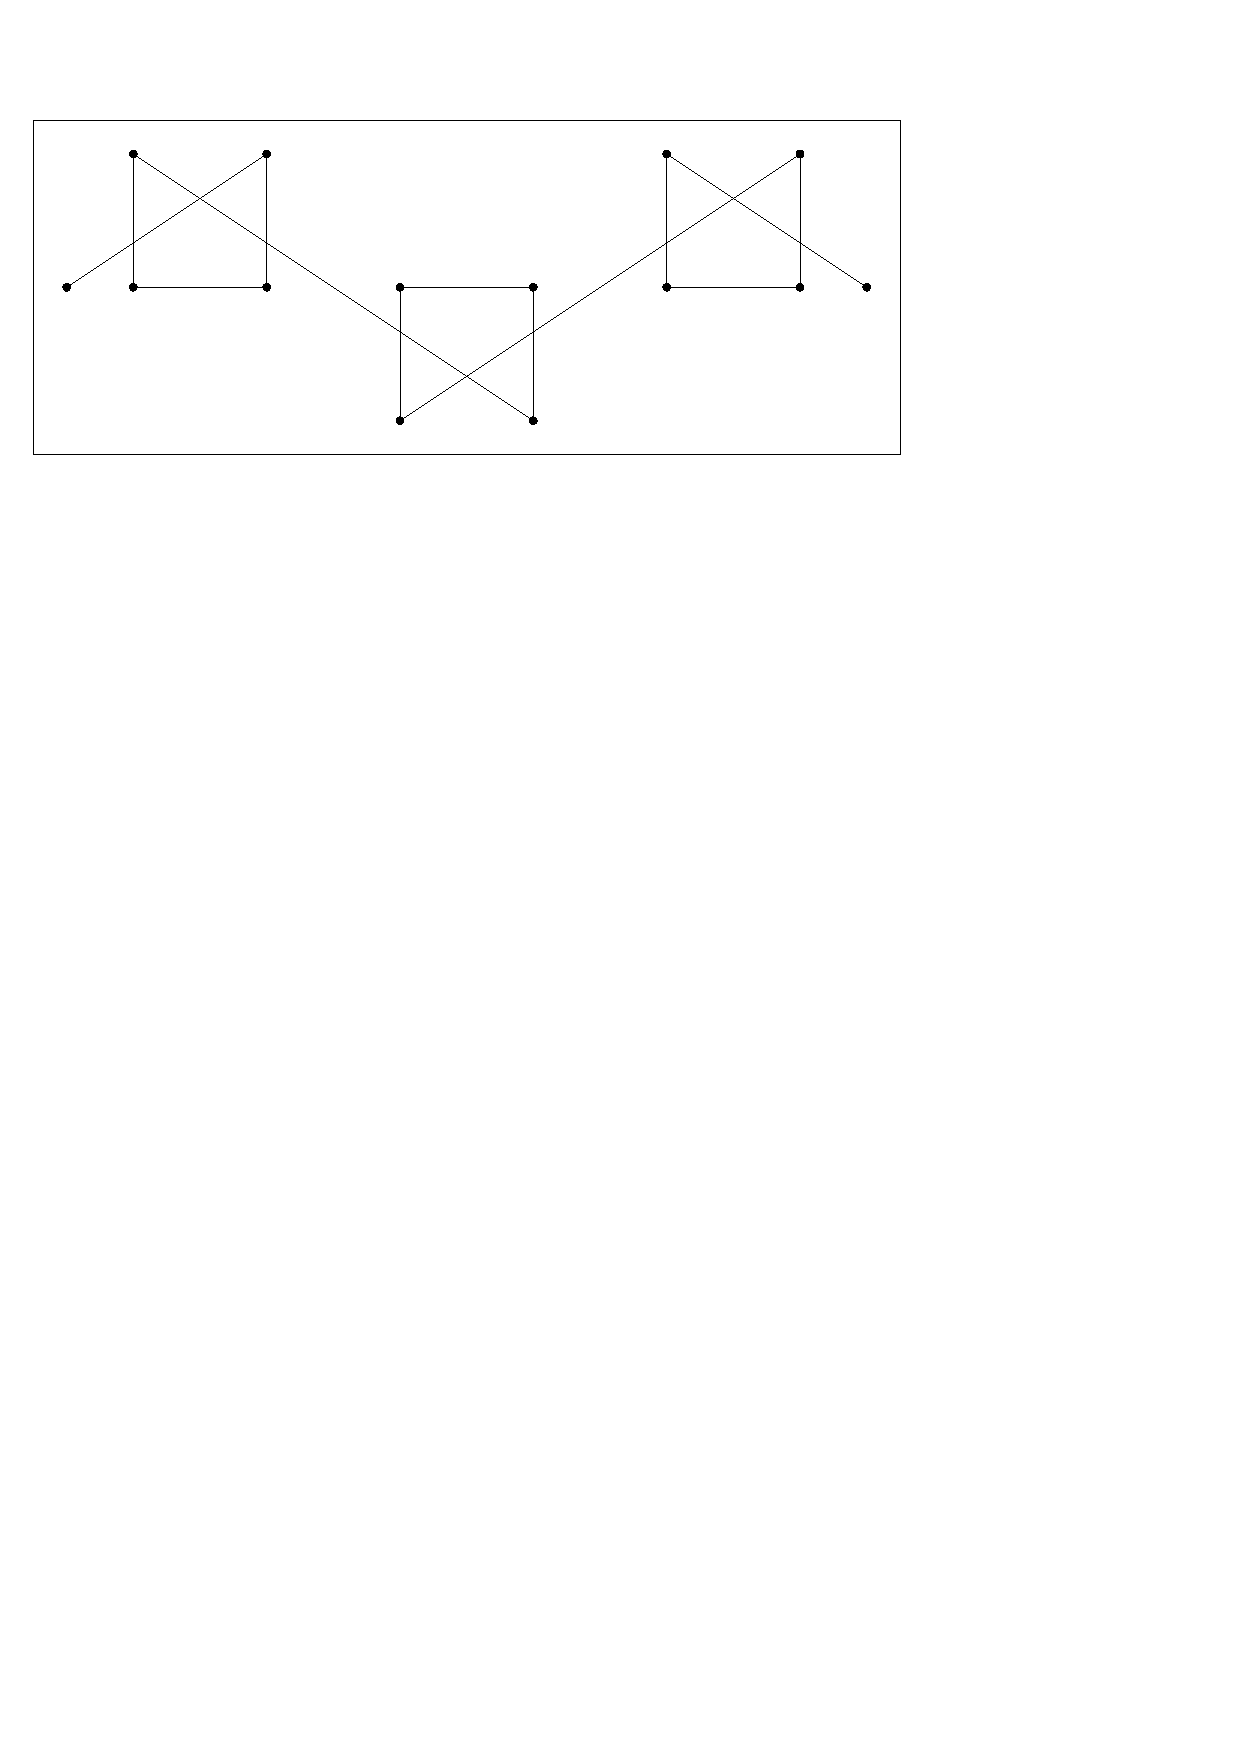
\includegraphics[scale=1]{graphics/crossingEdgeLinkage.pdf}
\end{center} 
\caption{A linkage where edges cross however it does not contain loops or multiple edges between 
vertices.}
\label{fig:linkage-3}
\end{figure}